\documentclass[
	12pt,
	]{article}
		\usepackage{xcolor}
			\usepackage[dvipsnames]{xcolor}
			\usepackage[many]{tcolorbox}
		\usepackage{changepage}
		\usepackage{titlesec}
		\usepackage{caption}
		\usepackage{mdframed, longtable}
		\usepackage{mathtools, amssymb, amsfonts, amsthm, bm,amsmath} 
		\usepackage{array, tabularx, booktabs}
		\usepackage{graphicx,wrapfig, float, caption}
		\usepackage{tikz,physics,cancel, siunitx, xfrac}
		\usepackage{graphics, fancyhdr}
		\usepackage{lipsum}
		\usepackage{xparse}
		\usepackage{thmtools}
		\usepackage{mathrsfs}
		\usepackage{undertilde}
		\usepackage{tikz}
		\usepackage{fullpage,enumitem}
		\usepackage[labelfont=bf]{caption}
	\newcommand{\td}{\text{dim}}
	\newcommand{\tvw}{T : V\xrightarrow{} W }
	\newcommand{\ttt}{\widetilde{T}}
	\newcommand{\ex}{\textbf{Example}}
	\newcommand{\aR}{\alpha \in \mathbb{R}}
	\newcommand{\abR}{\alpha \beta \in \mathbb{R}}
	\newcommand{\un}{u_1 , u_2 , \dots , n}
	\newcommand{\an}{\alpha_1, \alpha_2, \dots, \alpha_2 }
	\newcommand{\sS}{\text{Span}(\mathcal{S})}
	\newcommand{\sSt}{($\mathcal{S}$)}
	\newcommand{\la}{\langle}
	\newcommand{\ra}{\rangle}
	\newcommand{\Rn}{\mathbb{R}^{n}}
	\newcommand{\R}{\mathbb{R}}
	\newcommand{\Rm}{\mathbb{R}^{m}}
	\usepackage{fullpage, fancyhdr}
	\newcommand{\La}{\mathcal{L}}


	\usepackage{mathtools}
	\DeclarePairedDelimiter{\norm}{\lVert}{\rVert}
	\newcommand{\vectorproj}[2][]{\textit{proj}_{\vect{#1}}\vect{#2}}
	\newcommand{\vect}{\mathbf}
	\newcommand{\uuuu}{\sum_{i=1}^{n}\frac{<u,u_i}{<u_i,u_i>} u_i}
	\newcommand{\B}{\mathcal{B}}
	\newcommand{\Ss}{\mathcal{S}}
	
	\newtheorem{theorem}{Theorem}[section]
	\theoremstyle{definition}
	\newtheorem{corollary}{Corollary}[theorem]
	\theoremstyle{definition}
	\newtheorem{lemma}[theorem]{Lemma}
	\theoremstyle{definition}
	\newtheorem{definition}{Definition}[section]
	\theoremstyle{definition}
	\newtheorem{Proposition}{Proposition}[section]
	\theoremstyle{definition}
	\newtheorem*{example}{Example}
	\theoremstyle{example}
	\newtheorem*{note}{Note}
	\theoremstyle{note}
	\newtheorem*{remark}{Remark}
	\theoremstyle{remark}
	\newtheorem*{example2}{External Example}
	\theoremstyle{example}
	
	\title{MATH 325 Ass 5.}
	\titleformat*{\section}{\LARGE\normalfont\fontsize{12}{12}\bfseries}
	\titleformat*{\subsection}{\Large\normalfont\fontsize{10}{15}\bfseries}
	\author{Mihail Anghelici 260928404 }
	\date{\today}
	
	\relpenalty=9999
			\binoppenalty=9999
		
			\renewcommand{\sectionmark}[1]{%
			\markboth{\thesection\quad #1}{}}
			
			\fancypagestyle{plain}{%
			  \fancyhf{}
			  \fancyhead[L]{\rule[0pt]{0pt}{0pt} Assignment 5} 
			  \fancyhead[R]{\small Mihail Anghelici $260928404$} 
			  \fancyfoot[C]{-- \thepage\ --}
			  \renewcommand{\headrulewidth}{0.4pt}}
			\pagestyle{plain}
			\setlength{\headsep}{1cm}
	\captionsetup{margin =1cm}
	\begin{document}
	\maketitle
		\section*{Question 1}
			We note that since $p(x) = 0 \implies p_n = 0 \ \forall \ n \ge 0$. Also, $q(x) = k^{2}t^{2} \implies q_n =0 \ \forall \ n \ge  k^{2}t^{2}.$ Using the recursive formula we have 
			\begin{align*}
				a_{n+2} &= \frac{-1}{(n+2)(n+1)} \sum_{k \ge 0} (k+1) a_{k+1}p_{n-k} + a_{k}q_{n-k}\\
				&=\frac{-1}{(n+2)(n+1)} \sum_{k \ge 0} a_{k}q_{n-k} = \frac{-a_{n}k^{2}t^{2}}{(n+2)(n+1)} \quad \forall \  n \ge 0.
			\end{align*}
			\begin{equation*}
				\vrule \: \vrule  \begin{minipage}{0.4\linewidth}
					\begin{align*}
						a_{2} &= \frac{-a_{0}k^{2}t^{k}}{2!}\\
						a_{4} &= \frac{-a_{0}k^{4}t^{4}}{24} \\
						a_{6} &= \frac{-a_{0}k^{6}t^{6}}{(30)(12)(2)}
					\end{align*}	
				\end{minipage} \ \ \vrule 
				\begin{minipage}{0.4\linewidth}
					\begin{align*}
											a_{3} &= \frac{-a_{1}k^{2}t^{k}}{6}\\
											a_{5} &= \frac{a_{1}k^{4}t^{4}}{120} \\
											a_{7} &= \frac{-a_{1}k^{6}t^{6}}{(120)(60)}
										\end{align*}
				\end{minipage}\vrule  \: \vrule 
			\end{equation*}
			This leads to the recursion relationship 
			\begin{align*}
				&\textbf{EVEN} : a_{n} = a_{2j} = \frac{(-1)^{j}a_{0}k^{2j}t^{2j}}{(2j)!} ,\quad j\ge 1, \quad 
				\textbf{ODD} : a_{n} = a_{2j+1} = \frac{(-1)^{j} a_{1} k^{2j}t^{2j}}{(2j+1)!} \quad j \ge 1.
			\end{align*}
			\begin{align*}
				\therefore y(x) &= a_{0}\left(\sum_{j \ge 0} \frac{(-1)^{j} k^{2j} t^{2j} x^{2j}}{(2j)!}\right) + a_{1}\left(\sum_{j \ge 0} \frac{(-1)^{j}k^{2j}t^{2j}x^{2j+1}}{(2j+1)!}\right) \\
				 &= a_{0}\left(\sum_{j \ge 0} \frac{(-1)^{j} k^{2j} t^{2j} x^{2j}}{(2j)!}\right) + \frac{a_{1}}{kt}\left(\sum_{j \ge 0} \frac{(-1)^{j}k^{2j+1}t^{2j+1}x^{2j+1}}{(2j+1)!}\right) \\
				 &= a_{0}\cos(ktx) + \frac{a_{1}}{kt} \sin(ktx) 
				 \intertext{Using the initial conditions we replace the coefficients $a_{0}$ and $a_{1}$ yielding the final expression} 
				 y(x) &= y_{0}\cos(ktx) + \frac{y'_{0}}{kt} \sin(ktx).
			\end{align*}
			
			\section*{Question 2}
				We first and foremost note that $p(x) = x \implies p_{0} = x \implies p_{n} = 0 \ \forall \ n \ge x$. Moreover, $q(x) = 2 \implies q_{n} = 0 \ \forall \ n\ge 2 \implies q_{0} = 2.$ We'll solve the given IVP by using the differentiating method of the power series.
				
				$$y = \sum_{k \ge 0}a_{n}x^{n}, \qquad  xy' = \sum_{k \ge 1} na_{n}x^{n}, \qquad y'' = \sum_{k \ge 0} (n+2)(n+1)a_{n+2}x^{n}.$$
				\begin{align*}
					\therefore y(x) &= \sum_{k \ge 0} (n+2)(n+1)a_{n+2}x^{n} + \sum_{k \ge 1} na_{n}x^{n} + 2\sum_{k \ge 0}a_{n}x^{n} =0 \\
					&= a_{2}(2)(1) +  \sum_{k \ge 1} (n+2)(n+1)a_{n+2}x^{n} +  \sum_{k \ge 1} na_{n}x^{n} + 2a_{0} + \sum_{k \ge 1}2a_{n}x^{n} =0\\
					&= 2(a_{2}+a_{0}) + \sum_{k \ge 1}\left(((n+2)(n+1)a_{n+2}+na_{n} +2a_{n})x^{n}\right) = 0
					\intertext{$\because$ linear independence, }
					&a_{2}+a_{0}= 0 \implies a_{2} = -a_{0} \quad \text{and} \quad ((n+2)(n+1)a_{n+2}+na_{n} +2a_{n})x^{n} =0 \\
					&\qquad \qquad \therefore a_{n+2} = \frac{-a_{n}(n+2)}{(n+2)(n+1)} = \frac{-a_{n}}{n+1} \quad , n\ge 1.
				\end{align*}
				\begin{equation*}
								\vrule \: \vrule  \begin{minipage}{0.4\linewidth}
									\begin{align*}
										a_{2} &= \frac{-a_{0}}{1}\\
										a_{4} &= \frac{a_{0}}{3} \\
										a_{6} &= \frac{a_{0}}{15}
									\end{align*}	
								\end{minipage} \ \ \vrule 
								\begin{minipage}{0.4\linewidth}
									\begin{align*}
															a_{3} &= \frac{-a_{1}}{2}\\
															a_{5} &= \frac{a_{1}}{8} \\
															a_{7} &= \frac{-a_{1}}{48}
														\end{align*}
								\end{minipage}\vrule  \: \vrule 
							\end{equation*}
						This leads to the recursion relationship 
				\begin{align*}
								&\textbf{EVEN} : a_{n} = a_{2k} = \frac{(-1)^{k}a_{0}2^{k}k!}{(2k)!} \quad k \ge 1,\quad 
								\textbf{ODD} : a_{n} = a_{2k+1} = \frac{(-1)^{k} a_{1}}{2^{k}k!} \quad k\ge 1.
							\end{align*}
				Finally, 
				\begin{align*}
					y(x) &= a_{0}\sum_{k \ge 0} \frac{(-1)^{k}2^{k}k!x^{2k}}{(2k)!} + a_{1}\sum_{k \ge 0}\frac{(-1)^{k}x^{2k+1}}{2^{k}k!} \\
					\intertext{Using the initial conditions we may replace $a_{0}$ and $a_{1}$, giving}
					&= -3 \sum_{k \ge 0 } \frac{(-1)^{k}2^{k}k!x^{2k}}{(2k)!} + 2\sum_{k \ge 0}\frac{(-1)^{k}x^{2k+1}}{2^{k}k!}.
				\end{align*}
				\begin{figure}[H]
					\centering 
					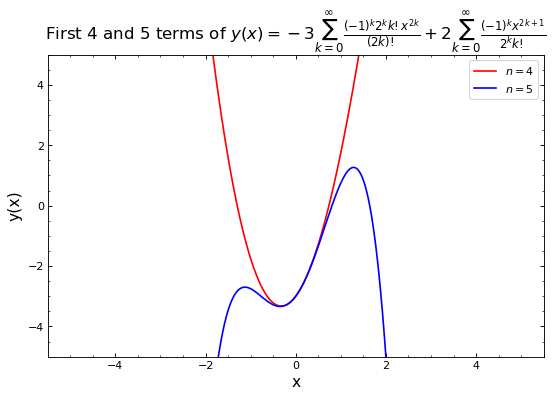
\includegraphics[width=0.9\linewidth]{MATH325_Ass5_Fig.png}
					\captionsetup{margin=1.5cm , justification=raggedright} \caption{First 4 and 5 term approximation to the solution of Question 2.}
				\end{figure}	
				
				\section*{Question 3}
				Due to confusion about the problem statement, I will provide two methods for finding the first three coefficients. \\
				
				\noindent \textbf{(METHOD 1)} : The given IVP is exact thus\\ 
					\begin{align*}
					\int \frac{dy}{\sqrt{1-y^2}} &= \int dx \\
					\sin^{-1}(y) &= x+C,
					\end{align*}
					given the initial condition $y(0)=0$, 
					\begin{gather*}
					y = \sin(x+0) = \sin(x)\\
					\therefore y(x) = \sum_{k\ge 0} \frac{(-1)^k x^{2k+1}}{(2k+1)!} = x - \frac{x^3}{3!} + \dots.
					\end{gather*}
					Therefore,using the initial condition $a_{0} = 0$, the coefficients up to $x^3$ as requested are $\{0,1,0, -\frac16 \}$. \\
					
					\noindent \textbf{(METHOD 2)} : 
					Let $y(x)$ be analytic. Then it follows that 
					\begin{align*}
						y(x) &=a_{0}+ a_{1}x + a_{2}x^{2} + a_{3}x^{3} + O(x^{4}) 
						\intertext{Since $a_{0} = 0$ ,}
						&= a_{1}x + a_{2}x^{2} + a_{3}x^{3} + O(x^{4}) \\
						\implies y'(x) &= a_{1} + 2a_{2}x + 3a_{3}x^{2} + O(x^{3})
						\intertext{Replacing in $y'=  \sqrt{1-y^{2}}$ yields} 
						y'(x) &= \sqrt{1 - (a_{1}x + a_{2}x^{2} + O(x^{3}))^{2}}\\
						&= \sqrt{1- (a_{1}x^{2} + 2a_{1}a_{2}x^{3} + O(x^{4}))}
						\intertext{We may now use the Taylor expansion for $\sqrt{1-x}$,}
						&= 1- \frac12(a_{1}^{2}x^{2} + 2a_{1}a_{2}x^{3} +O(x^{4}) )
						\intertext{Since we need the coefficients up to $x^{3}$ this reduces to }
						y'(x) &= 1 -\frac12 a_{1}^{2}x^{2} + O(x^{3}) \\
						\therefore a_{1} + 2a_{2}x + 3a_{3}x^{2} + O(x^{3}) &= 1-\frac12 a_{1}^{2}x^{2} + O(x^{3}) \\
						\implies (a_{1}-1) + 2a_{2}x &+ \left(3a_{3}+ \frac12 a_{1}^{2}\right)x^{2} = 0
						\intertext{$\because$ linear independence, }
						\implies a_{1} = 1\quad ,&a_{2} =0 \quad, a_{3} = -\frac16.
					\end{align*}
					We conclude that the coefficients up to $x^{3}$ are $\{0,1,0,-\frac16\}$. 
				\section*{Question 4}
					\subsection*{a) }
						\begin{align*}
							(1-x^{2}) \sum_{n=0}^{\infty} n(n-1)a_{n}x^{n-2} -2x\sum_{n=0}^{\infty} n a_{n}x^{n-1} + \alpha(\alpha+1)\sum_{n=0}^{\infty} a_{n}x^{n} &= 0\\
							\sum_{n=0}^{\infty} n(n-1)a_{n}x^{n-2} - \sum_{n=0}^{\infty}n(n-1)a_{n}x^{n} - 2\sum_{n=0}^{\infty} n a_{n}x^{n} + \alpha(\alpha+1)\sum_{n=0}^{\infty}a_{n}x^{n} &= 0\\
							\sum_{n=0}^{\infty} (n+2)(n+1)a_{n+2}x^{n} \sum_{n=0}^{\infty}n(n-1)a_{n}x^{n} - 2\sum_{n=0}^{\infty} n a_{n}x^{n} + \alpha(\alpha+1)\sum_{n=0}^{\infty}a_{n}x^{n} &= 0 \\
							\implies \sum_{n=0}^{\infty} \left((n+2)(n+1)a_{n+2} - n(n-1)a_{n} -2na_{n} + \alpha(\alpha+1)a_{n}\right)x^{n} &= 0
							\intertext{By linear independence, }
						\end{align*}
						\vspace{-1.5cm}
						\begin{align*}
							\implies a_{n+2}  &= \frac{n(n-1)a_{n} + 2na_{n} - \alpha(\alpha+1)a_{n}}{(n+2)(n+1)} \\
							&= \frac{a_{n}((n-\alpha)(n+\alpha+1))}{(n+2)(n+1)} \quad n \ge 1.
						\end{align*}
					\begin{equation*}
												\vrule \: \vrule  \ \ \begin{minipage}{0.4\linewidth}
													\begin{align*}
														a_{2} &= \frac{a_{0}(-\alpha)(\alpha+1)}{2}\\
														a_{4} &= \frac{a_{0}(\alpha+1)(\alpha-2)(\alpha+3)}{4} \\
														a_{6} &= \frac{a_{0}-(\alpha+1)(\alpha-2)(\alpha+3)(\alpha-4)(\alpha+5)}{6!}
													\end{align*}	
												\end{minipage} \ \  \vrule \ \
												\begin{minipage}{0.4\linewidth}
													\begin{align*}
																			a_{3} &= \frac{-a_{1}(\alpha-1)(\alpha+2)}{3!}\\
																			a_{5} &= \frac{a_{1}(\alpha-1)(\alpha+2)(\alpha-3)(\alpha+4)}{8} \\
																			a_{7} &= \frac{-a_{1}(\alpha-1)(\alpha+2)(\alpha-3)(\alpha+4)(\alpha-5)(\alpha+6)}{7!}
																		\end{align*}
												\end{minipage}\vrule  \: \vrule 
											\end{equation*}	
							This leads to the recursion relationship 
									\begin{align*}
													&\textbf{EVEN} : a_{n} = a_{2k} = \frac{(-1)^{k}a_{0}\alpha (\alpha+2k-1)(\alpha+2k-3)\dots(\alpha+1)(\alpha-2)\dots(\alpha-2k+2)}{(2k)!}  , \ k\ge 1\\
													&\textbf{ODD} : a_{n} = a_{2k+1} = \frac{(-1)^{k} a_{1}(\alpha+2k)(\alpha+2k-2)\dots(\alpha+2)(\alpha-1)\dots(\alpha-2k+1)}{(2k+1)!} \ \ ,k \ge 1.
												\end{align*}
					Therefore we write the series solution as
					\begin{gather*}
						y(x) = y_{0} y_1(x) + y_{0}' y_2(x),\\
						\text{where } \quad y_{1}(x) = 1 + \sum_{k=1}^{\infty}\frac{(-1)^{k}a_{0}\alpha (\alpha+2k-1)(\alpha+2n-3)\dots(\alpha+1)(\alpha-2)\dots(\alpha-2k+2)}{(2k)!} \\
						\text{and} \quad y_{2}(x) = x + \sum_{k=0}^{\infty} \frac{(-1)^{k} a_{1}(\alpha+2k)(\alpha+2k-2)\dots(\alpha+2)(\alpha-1)\dots(\alpha-2k+1)}{(2k+1)!}
					\end{gather*}
				\subsection*{b) }
					Letting $\alpha = 2k$, all the terms after the $k$th term are terminated since they contain the factor $\alpha-2k$, therefore since the $k$th term has the highest power in $x$, that term will dictate the degree of the polynomial ,i.e., $2k$.\\ 
					
					\noindent Similarly, if $\alpha =2k+1$ then all the terms which contain $\alpha-(2k+1)$ will vanish ,leaving the $k$th term having the power of $2k+1$ such that $\text{deg}(y_{2}(x)) = 2k+1$.
					
					\begin{equation*}
						\vrule \ \vrule \ \begin{minipage}{0.4\linewidth}
							\begin{alignat*}{2}
								y_{1}(x) &= 1 &&,(\alpha=0)\\
								y_{1}(x) &= 1-3x^{2} &&,(\alpha=2)\\
								y_{1}(x) &= 1-10x^{2}+\frac{35}{3}x^{4} && ,(\alpha=4) 
							\end{alignat*}
						\end{minipage}
						\ \ \vrule \ \
						\begin{minipage}{0.4\linewidth}
							\begin{alignat*}{2}
								y_{2}(x) &= x &&, (\alpha=1)\\
								y_{2}(x) &= x-\frac53 x^{3} && ,(\alpha=3)\\
								y_{2}(x) &= x-\frac{14}{3}x^{3} + \frac{21}{5}x^{5} && ,(\alpha=5) 
							\end{alignat*}							
						\end{minipage}
						\ 	\vrule \ \vrule \
					\end{equation*} 
				\subsection*{c) }
					\begin{alignat*}{4}
						&\boldsymbol{(\alpha =0)}\quad & \quad  &1 \quad : &P_{0}(1) = 1 \implies P_{0}(x) = 1 \checkmark \\
						&\boldsymbol{(\alpha=1)}\quad & \quad  &x \quad : &P_{1}(1) =1 \implies P_{1}(x) = x \checkmark \\
						&\boldsymbol{(\alpha=2)}\quad & \quad  &1-3x^{2} \quad : &P_{2}(1) =-2 
						\intertext{ a(1-3) =1 \implies a = -\dfrac12 \ \ \therefore  P_{2}(x) = \dfrac{3x^{2}-1}{2} \ \checkmark. }
						&\boldsymbol{(\alpha=3)}\quad & \quad  &x- \frac{5}{3}x^{3} \quad : &P_{3}(1) \neq 1
						\intertext{ a\left(1-\dfrac53\right)=1 \implies a = -\dfrac32 \ \ \therefore P_{3}(x) = \dfrac{5x^{3}-3x}{2} \ \checkmark.}
						&\boldsymbol{(\alpha=4)} \quad & \quad &1-10x^{2} +\frac{35}{3}x^{4} \quad &P_{4}(1) \neq 1 
						\intertext{a\left(1-10+\dfrac{35}{3}\right) =1 \implies a = \dfrac38  \ \ \therefore P_{4}(x) = \dfrac{35x^{4} -30x^{2}+3}{8}  \ \checkmark.}
						&\boldsymbol{(\alpha=5)} \quad & \quad &x-\frac{14}{3}x^{3} + \frac{21}{5}x^{5} \quad &P_{5}(1) \neq 1 
						\intertext{a\left(1-\dfrac{14}{3} + \dfrac{21}{5}\right)=1 \implies a = \dfrac{15}{8} \ \ \therefore P_{5}(x) = \dfrac{63x^{5}-70x^{3}+15x}{8} \ \checkmark.}
					\end{alignat*}
			\section*{Question 5}
				\begin{equation*}
					y_{n+1} = y_{n} + h \begin{pmatrix}
						(y_{1})_{n} (a-\alpha y_{2}) \\ (y_{2})_{n} (-c + \gamma y_{1}).
					\end{pmatrix}
				\end{equation*}
				\begin{figure}[H]
					\centering 
					\includegraphics[width = 0.8\linewidth]{MATH325_Ass5_Fig2.png}
					\captionsetup{margin=1.5cm ,justification = raggedright}
					\caption{Euler's method applied to Lotka-Volterra biological model with $a,b,\alpha, \gamma = 1,1/2, 3/4, 1/4$, respectively.}
				\end{figure}
				\vspace{-0.6cm}
				\begin{enumerate}[label=(\alph*)]
					\color{red} \item \color{black} In the absence of prey, the population of predators decrease exponentially since the interaction between the two populations is null and the death rate is negative. The number of predators start at $3$ individuals as defined in the initial condition and converge to $0$ as the time approaches infinity 
					\color{blue} \item  \color{black} In the absence of predators, the population of prey increase exponentially since the interaction between the two populations is positive but small and the growth rate is positive. The number of prey start at $3/10000$ individuals as defined in the initial condition and increase exponentially up to $\approx 6.7$ given that $10000$ cycle iterations are performed on the population, but would go indefinitely further given a larger number of iterations.
					\item  IF there are initially $2$ prey and $2$ predators , the biological system will oscillate over time. The growth and death rate of the two species are inversely proportional to one other such that one species is striving while the other is not and the roles interchange consistently over time. 
					\color{green} \item \color{black} If there are initially $3$ prey and $2$ predators, the biological system will remain constant over time. This means that the growth rate of prey and the death rate of the predators are both null since both species are ,within this model, mutually sustainable. 
				\end{enumerate}
	\end{document}